\documentclass[12pt]{article}
\setlength{\oddsidemargin}{0in}
\setlength{\evensidemargin}{0in}
\setlength{\textwidth}{6.5in}
\setlength{\parindent}{0in}
\setlength{\parskip}{\baselineskip}
\usepackage{amsmath,amsfonts,amssymb}
\usepackage{graphicx}
\usepackage[]{algorithmicx}
\usepackage{enumitem}
\usepackage{fancyvrb}
\usepackage{setspace}
\usepackage[]{algorithm2e}
\usepackage{fancyhdr}
\pagestyle{fancy}
\setlength{\headsep}{36pt}

\usepackage{hyperref}

\hypersetup{
    colorlinks=true,
    linkcolor=blue,
    filecolor=magenta,      
    urlcolor=blue,
}

\newcommand{\makenonemptybox}[2]{%
%\par\nobreak\vspace{\ht\strutbox}\noindent
\item[]
\fbox{% added -2\fboxrule to specified width to avoid overfull hboxes
% and removed the -2\fboxsep from height specification (image not updated)
% because in MWE 2cm is should be height of contents excluding sep and frame
\parbox[c][#1][t]{\dimexpr\linewidth-2\fboxsep-2\fboxrule}{
  \hrule width \hsize height 0pt
  #2
 }%
}%
\par\vspace{\ht\strutbox}
}
\makeatother

\begin{document}
\lhead{{\bf CSCI 3104, Algorithms \\ Final Exam Summer 2020 (60 points)  } }
\rhead{Name: \fbox{% Place your name here and delete the next time
\phantom{This is a really long name}} 
\\ ID: \fbox{ %+ Place your ID here and delete the next time
\phantom{This is a student ID}} 
\\ {\bf Escobedo \& Jahagirdar\\ Summer 2020, CU-Boulder}}
\renewcommand{\headrulewidth}{0.5pt}

\phantom{Test}

\begin{figure}[h!]
    \begin{center}
    \includegraphics[scale=0.15]{Final/dont_panic.png} 
    \end{center}
    \end{figure}
\begin{small}


\textit{Advice 1}:\ For every problem in this class, you must justify your answer:\ show how you arrived at it and why it is correct. If there are assumptions you need to make along the way, state those clearly.
%\vspace{-3mm} 

\textit{Advice 2}:\ Verbal reasoning is typically insufficient for full credit. Instead, write a logical argument, in the style of a mathematical proof.\\
%\vspace{-3mm} 

\textbf{Honor code}: On my honor as a University of Colorado at Boulder student,
I have neither given nor sought unauthorized assistance in this work\\  \\
\textbf{Initials} 
\fbox{% Place your iniitals here and delete the next time
\phantom{This is a really long name}} \\ \\
\textbf{Date} 
\fbox{% Place your Date here and delete the next time
\phantom{This is a really long name}} \\ 


If you violate the CU \textbf{Honor Code}, you will receive a 0.
\clearpage
\textbf{Instructions for submitting your solution}:
\vspace{-5mm} 

\begin{itemize}
	\item The solutions \textbf{should be typed}, we cannot accept hand-written solutions. Here's a short intro to \href{http://ece.uprm.edu/~caceros/latex/introduction.pdf}{\textbf{Latex}.}
	 \item In this homework we denote the asymptomatic \textit{Big-O} notation by $\mathcal{O}$ and \textit{Small-O} notation is represented as $o$. 
	\item We recommend using online Latex editor \href{https://www.overleaf.com/}{\textbf{Overleaf}}. Download the \textbf{.tex} file from Canvas and upload it on overleaf to edit.
	%todo add link of gradescope
	\item You should submit your work through \href{https://www.gradescope.com}{\textbf{Gradescope}}  only.
	\item If you don't have an account on it, sign up for one using your CU email. You should have gotten an email to sign up. If your name based CU email doesn't work, try the identikey@colorado.edu version. 
	\item Gradescope will only accept \textbf{.pdf} files (except for code files that should be submitted separately on Canvas if a problem set has them) and \textbf{try to fit your work in the box provided}. 
	\item You cannot submit a pdf which has less pages than what we provided you as Gradescope won't allow it.
   
\end{itemize}
\vspace{-4mm} 
\end{small}
\clearpage

%\hrulefill





\begin{enumerate}


	
	
	
	\item{
	    (5 pts) You are given a list of jobs with start and end times. Assume that only one job can be executed at a time on a processor. Your task is to find out the minimum number of processors required so that the jobs are  executed as soon as they arrive (no waiting time for a process).
	    The input to your algorithm will be a list of tuples indicating the start and end times of the respective jobs. The output should be a number indicating the minimum number of processors required. Your algorithm should have a runtime of $\mathcal{O}(n \log(n))$, where $n$ is the number of jobs. Assume you do not have access to any auxiliary functions.\\
	    
	    \textbf{Example} \\
        \textbf{Input}: $(2, 10) , (9, 11), (15, 18), (3, 4), (17, 19), (5, 13)$ \\
        \textbf{Output}: $3$ \\
        \textbf{Explanation}: Between the interval $(9, 10)$ it can be seen that there will be 3 \{ (2, 10) , (9, 11),  (5, 13)\} jobs that need to be executed simultaneously. Thus at the very least 3 processors are required. \\ 
        
        \begin{enumerate}
	        \item (4 pts) Write down well commented pseudo-code or paste real code to solve the above problem.
	        \makenonemptybox{5in}{ 
	        	\begin{algorithmic}


	        		
	        		\State processes$\gets$$phi$ \Comment{It is of list of processe}
	        		\State st$\gets$ $phi$ \Comment{ st is array of starting time }

	        		\State et$\gets$ $phi$ \Comment{ et is array of ending time }
	        		\State \For{(i,j in process)}
	        	{Append st using i and append st using j}
	        	\EndFor
	        	
	        	\Comment{Sort both st,et in increasing order}
	        \State \text{cur\_proc}$\gets$1,result$\gets$1 
	        \State i$\gets$1 and j$\gets$0
	        \State Loop{i and j less than proc size}{\State \If{st[i]$\leq$et[i]}{Increment \text{cur\_proc} and i by 1}\ElseIf{st[i]>et[j]}{Decrement \text{cur\_proc} and increment j }\EndIf
	        	\State \If{\text{cur\_proc}>result}{result$\gets$\text{cur\_proc}}\EndIf}
	        	\State print result
	        
        
    
	        \end{algorithmic}}
	        \clearpage
	        \item (1 pts) Explain your algorithms runtime and space complexity by analyzing your code. For example, stating that a sorting algorithm runs in $\mathcal{O}(n \log(n))$ without any justification is insufficient. 
	        \makenonemptybox{3in}{Time Complexity: O(n Log n).

	        	Sorting takes N log N and single traversal of an array takes O(n).
Time Complexity:$\mathcal{O}(n \log(n))$+$O(n)$ = $\mathcal{O}(n \log(n))$ \\
	        	Space Complexity: O(1).

	        	As no extra space is required.}
	    \end{enumerate}
	}
	
	\clearpage
	
	\item{
	    (5 pts) You are designing a network, to connect several offices in different locations. You can contact your network cable provider about the cost of connecting any pair of offices. Your task is to design an algorithm, so that all offices are connected and the cost associated with building the network is minimized.\\
	    The input to your algorithm is a Graph in the form of an adjacency list or matrix. The nodes in this graph represent the offices and edge weights represent the cost associated with connecting a pair of offices. The output of the algorithm will be a list of office pairs such that the total connection cost is minimized. \\
	    \begin{enumerate}
	        \item (2 pts) Provide an example with at least 3 offices and 3 connections. Your example must include at least 2 unique solutions.
	        \makenonemptybox{4in}{offices = \begin{center}

	        		\begin{tabular}{ |c|c|c|c|c| } 

	        			\hline

	        			0&1&2&3&4\\
	        			\hline

	        			1& 0& 5& 0& 7\\ \hline  

	        			2&5&0&6&0 
\\ \hline 
	        			3&0& 6& 0& 0 \\ \hline 

	        			4&7& 0& 0&0  \\ \hline
	        		\end{tabular}

	        	\end{center}                                                                                                                 

	   min cost required = 10}
	        \clearpage
	       
	        \item (6 pts) Provide well commented pseudo code or actual code to solve the above problem.
	       % \makenonemptybox{6in}{
	        	\begin{verbatim}
	        	    # Function to find out minimum valued  

	        	# node among the nodes which are not  

	        	# yet included in MST  

	        	def minnode(n, keyval, mstset): 

	        	mini = 999999999999

	        	mini_index = None

	        	
	        	# Loop through all the values of  

	        	# the nodes which are not yet  

	        	# included in MST and find the  

	        	# minimum valued one. 

	        	for i in range(n): 

	        	if (mstset[i] == False and 

	        	keyval[i] < mini):  

	        	mini = keyval[i] 

	        	mini_index = i 

	        	return mini_index 

	        	
	        	# Function to find out the MST and  

	        	# the cost of the MST.  

	        	def findcost(n, Offices): 

	        	
	        	# Array to store the parent  

	        	# node of a particular node.  

	        	parent = [None] * n 

	        	
	        	# Array to store key value  

	        	# of each node.  

	        	keyval = [None] * n  

	        	
	        	# Boolean Array to hold bool  

	        	# values whether a node is 

	        	# included in MST or not.  

	        	mstset = [None] * n 

	        	\newpage
	        	# Set all the key values to infinite and  

	        	# none of the nodes is included in MST. 

	        	for i in range(n): 

	        	keyval[i] = 9999999999999

	        	mstset[i] = False

	        	
	        	# Start to find the MST from node 0.  

	        	# Parent of node 0 is none so set -1.  

	        	# key value or minimum cost to reach  

	        	# 0th node from 0th node is 0.  

	        	parent[0] = -1

	        	keyval[0] = 0

	        	
	        	# Find the rest n-1 nodes of MST. 

	        	for i in range(n - 1): 

	        	
	        	# First find out the minimum node  

	        	# among the nodes which are not yet  

	        	# included in MST.  

	        	u = minnode(n, keyval, mstset)  

	        	
	        	# Now the uth node is included in MST.  

	        	mstset[u] = True

	        	
	        	# Update the values of neighbor  

	        	# nodes of u which are not yet  

	        	# included in MST.  

	        	for v in range(n): 

	        	if (offices[u][v] and mstset[v] == False and 

	        	offices[u][v] < keyval[v]):  

	        	keyval[v] = offices[u][v]  

	        	parent[v] = u 

	        	
	        	# Find out the cost by adding  

	        	# the edge values of MST.  

	        	cost = 0

	        	for i in range(1, n): 

	        	cost += offices[parent[i]][i]

	        	print(parent[i],i) 

	        	print(cost) 

	        	
	        	
	        
	        	\end{verbatim}
	
	    \end{enumerate}
	   
	}
	
	\clearpage
	
	\item{
	    (10 pts) Consider the graph $G = (V, E)$ with edge capacities $c(e), \; \forall e \in E$, the edge capacity represents the maximum amount of flow that can pass through the edge. In addition to edge capacities, the above graph has vertex capacities $c(v), \; \forall v \in V - \{s, t\}$ (The source and the sink vertex do not have vertex capacities). Each vertex capacity represents the
	    maximum amount of flow that can pass through the vertex. \\
	     
	    
	    \begin{enumerate}
	        \item (4 pts) Given a source vertex $s \in V$ and a sink $t \in V$.  How will you modify the given graph $G$, so that you can find the max-flow from $s$ to $t$ with a known algorithm? Also, show an example input and modified graph with at least 5 vertices. This must be a drawing! 
	        \makenonemptybox{2in}{Since a flow graph has vertex capacity $c(v)$  flow $f(·,·)$is feasible only if, in addition to the flow constraints and the edge capacity constraints, it also satisfies the  vertex capacity constraint,\[
	        	\sum_{v:{u,v}\in E}{f(u,v)\leq c(v) \forall vertices in V}
	        	\]
       }
   \begin{figure}[h!]
   	\begin{center}
   		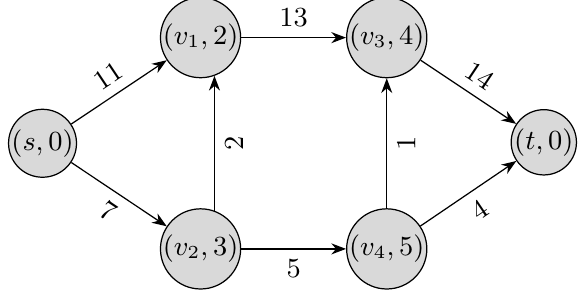
\includegraphics[scale=0.7]{/home/satyam/1595393986-Archive/HW7a1.png}
   	\end{center}
   \end{figure}
	        \clearpage
	        
	        \item (4 pts) Provide an algorithm to find the max-flow in the above graph from $s$ to $t$.
	        \makenonemptybox{2in}{
	        	This algorithm is slight modification of Ford-Fullerson's Algorithm.\\
	        	1) Initialize source and sink vertex capacity to 0. Start with initial flow as 0.

	        	
	        	2) While there is a augmenting path from source to sink.
	        		 Check the vertex capacity of all vertex from source to sink Take min of edge capacity and vertex capacity \\ 
	        		 Add this path-flow to flow.

	        	3) Return flow.}
	        
	        \item (2 pts) Find the max-flow in your example graph by stepping though your algorithm. Provide a new graph image each time the flow though an edge is altered. 
	         \begin{figure}[htp!]
	       	\begin{center}
	       		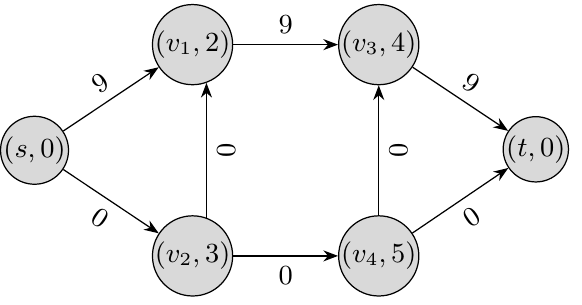
\includegraphics[scale=0.7]{/home/satyam/1595393986-Archive/HW7c.png}
	       	\end{center}
	       \end{figure}
	       \\Maximum flow through the network is 9
	    \end{enumerate}
	}
	
	\clearpage
	\item{
	    
	    (10 pts) There are $n$ rooms numbered from $\{1, 2, .. n\}$ in  Williams Village. Each of the rooms has a teleportation device with a value $v_i \; \; \forall i \in \{1, 2, ....n\}$. The teleportation device placed in the room $i$ with value $v_i$ teleports to a room numbered  $(v_i \; \% \; n) + 1$. 
	    
	    A room in Williams Village is said to be beautiful if you can get back to the room you started using the teleportation devices. The task is to count the number of beautiful rooms in Williams Village. \\
	    The input to your algorithm is the list of values associated with the teleportation device placed in the rooms. The output should be a number indicating the number of beautiful rooms. \\ \\
	    
	    \textbf{Example 1}\\
	    \textbf{Input}: [2, 3, 4, 5] \\
	    \textbf{Output}: 4\\
	    \textbf{Explanation}: All the 4 rooms that are beautiful and the corresponding paths  to get back to them are as follows.\\
	    \begin{itemize}
	        \item \textbf{Room 1} The teleportation path for Room1 is Room1, Room3, and back to Room1
	        \item \textbf{Room 2} The teleportation path for Room2 is Room2, Room4, and back to Room2
	        \item \textbf{Room 3} The teleportation path for Room3 is Room3, Room1, and back to Room3
	        \item \textbf{Room 4} The teleportation path for Room4 is Room4, Room2, and back to Room4
	    \end{itemize}
	    
	    \textbf{Example 2}\\
	    \textbf{Input}: [1, 2, 3, 6] \\
	    \textbf{Output}: 2\\
	    \textbf{Explanation}: It can be seen that only Room3 and Room4 are beautiful.
	    
	    \clearpage
	    \begin{enumerate}
	        \item (2 pts) Give a high-level explanation of how you plan to solve this problem. (How would you explain your potential solution to a younger sibling or someone who has never taken a computer science class?) Minimum 1 paragraph.
	        \makenonemptybox{3in}{Take 2 sets of equal points and label them as $R_{i}$ $\forall$ $i\in{1\cdots n}$. Map these sets  using the function $(v_i \; \% \; n) + 1$. If we see more than 1 path in any of the vertices in set 2 exclude that vertices from the set of input. We are always starting to count from the set 1. There exists a path from vertices in set 1 to set 2 and also from set 2 to set 1 of other vertices. This set of vertices is also excluded from the set.}
	        
	        \clearpage
	        \item (5 pts) Provide well commented pseudo code or actual code to solve the above problem.
	        \makenonemptybox{6in}{	Pseudo code for the following problem is as follows:
	        	\\If we get vertices (u,v) and (v,w), we will remove u from the first set.Apply DFS on the given set, which vertices selected from S1\\
	        	CountVertices is a function which takes 2 parameters $S1=(V,E)$ and $S2=(V',E')$, which are vertices of 2 sets, which will be used for mapping.
	        	\begin{algorithmic}


	        		\State \Function{Count Vertices} {$S1$, $S2$}
	        		\State count $\gets$ 0 \Comment{ Initial count = 0}

	        		\State visited[]$\gets$ False
	        		\State addVertex[] $\gets$ $\phi$
	        		\State \For{All vertices of Set 1 }
	        		{
	        			Mark the current vertices.
	        			visited[v] $\gets$ True
	        			\\Add vertices into addVertex[]
	        			\State \If{visited[v] is True in Set1 and visited[v] is False in set 2}{Increment Count}\EndIf
	        		}
	        		
	        	
	        		\State \Return count
	        		
	        		\EndFunction
	        	\end{algorithmic}
	        }
	        
	        \clearpage
	        \item (3 pts) Give an example input with at least 5 rooms and structure of how your algorithm explores the rooms. This must be an image! Your input can \textbf{not} be an example already given.
	        \makenonemptybox{3in}{Assume Input:[2,4,5,6,8]
	        \\Output:3(Room 4-Room 8 and back\\ Room 2 and Room 3 and back\\ Room 5 -Room 1 and back)}
         \begin{figure}[h!]
        	\begin{center}
        		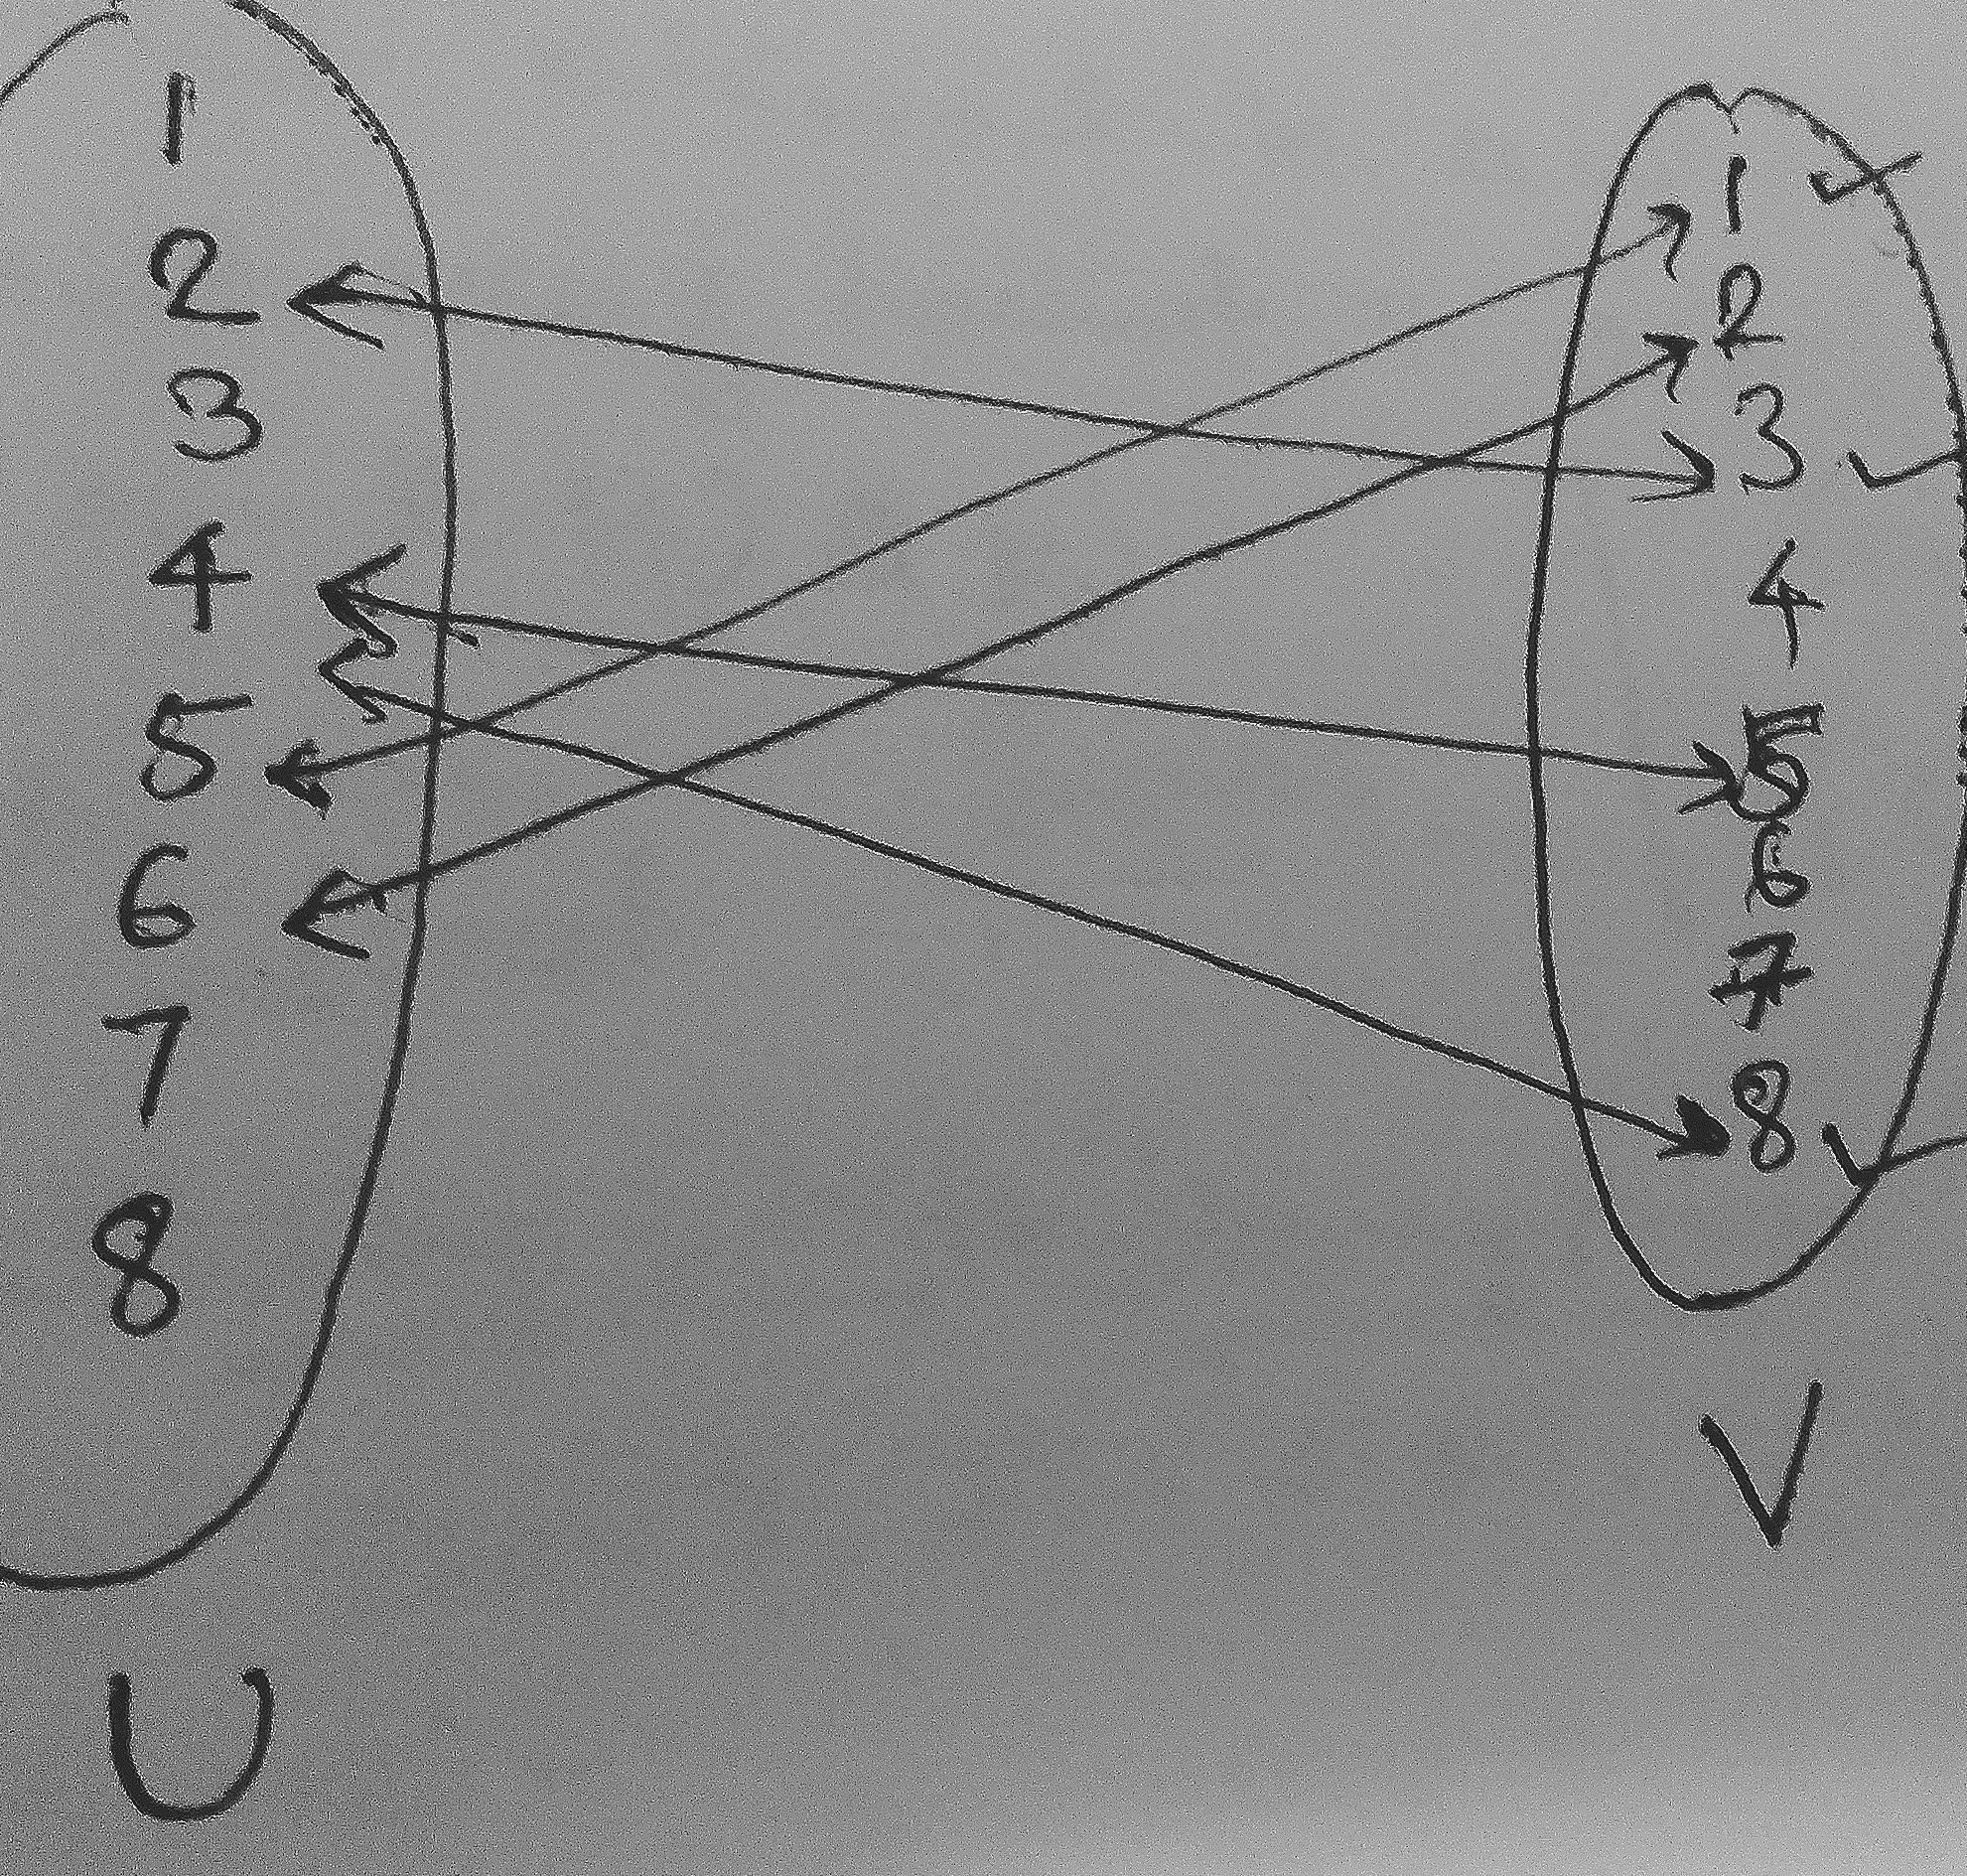
\includegraphics[scale=0.2]{/home/satyam/1595393986-Archive/HW5.jpg}
        	\end{center}
        \end{figure}
	    \end{enumerate}
	}
	
	\clearpage
	
	\item{
	    (10 pts) You are at your home in Boulder enjoying the summer and your friend challenges you to ride your bike for at least $s$ miles starting from your home and ending at any of the scenic outlooks. You have a map of Boulder that has information about roads connecting various view points and your house. The task is to determine if there is a sequence of scenic outlooks that you can travel to starting from your house such that you have travelled at least $s$ miles. You can not travel on the same edge more than 1 time and once you visit an outlook you cannot travel to it again.\\
	    The input to your problem is a graph $G=(V, E)$  in the form of an adjacency list or adjacency matrix and the source vertex $s$ corresponding to your house. Your algorithm should output a boolean value indicating if it's possible to complete the challenge of riding at least $s$ miles starting from your house.
	    
	    \begin{enumerate}
	        \item (2 pts) Give a high-level explanation of how you plan to solve this problem. (How would you explain your potential solution to a younger sibling or someone who has never taken a computer science class?) Minimum 1 paragraph. 
	        \makenonemptybox{4in}{Assume there are n points around your house. All the points are assumed to be scenic location in Boulder. Connect all this points starting from your house without lifting of your pencil/pen. The connection of this points will determine, whether it is less than s or greater than s, if all edges are assumed to be of weight 1. Every vertex will have even degree.}
	        \clearpage
	        
	        \item (6 pts) Provide well commented pseudo code or actual code to solve the above problem.
	        \makenonemptybox{6in}
	        {
	        	Pseudo code for the following problem is as follows:
	        	//If $G=(V,E)$ is a Euler graph, then keep on removing the edges from the graph and keep doing this distance of atleast s miles is not reached.
	        	
	        	\\Let find path be the function, which will take source u as the input parameter.\\
	      \begin{algorithmic}


	      	\State \Function{Find Path}{u}
	      	\State dist $\gets$ 0 \Comment{ source vertex distance = 0}

	      	\State addVertex[]
	      	\State \For{each edge e=(u,v) in E:}
	      	{ remove e from E\\Increment dist by 1\\
	     		 \Call {Find Path}{$u$}  and dist $<$ s\\ Update addVertex}
     		
      	\State	\EndFor
      		prepend u to addVertec\\
      	\Comment{The number of vertices added into u, gives the result of scenic location visited till dist s.}
	     \State 	\EndFunction
	      \end{algorithmic}
	        	
	        }
	        \clearpage
	        
	        \item (2 pts) Explain your algorithms runtime and space complexity by analyzing your code. For example, stating that a sorting algorithm runs in $\mathcal{O}(n \log(n))$ without any justification is insufficient. 
	        \makenonemptybox{3in}{Initializing dist and addVertex is $O(1)$. Loop runs over no of edges till dist of s ie $O(E)\timesO(1)$. Prepending takes $O(1)$.\\
	    $\therefore$ Time complexity is $O(1)$  + $O(E)$ + $O(1)$ = $O(E)$.
	    \\ Space Complexity: $O(E)$, as additional space of storing the edges is required.
        }
	        \clearpage
	    \end{enumerate}
	}
	
	\clearpage 
		\item{
    (20 pts) There are an even number of items arranged along a line. Each item has a value $v_i$ associated with it. You are competing against an opponent to collect items such that total value of your items collected is maximized. At each round of the game, one player is allowed to pick an item from either end of the line. \\ \\
    Determine the maximum total value that can be obtained, if you are allowed to play first assuming that the opponent is equally clever. The input to your algorithm will be a list of values. The output should be a number indicating the maximum amount of value that you can obtain.\\ 
    
    \textbf{Example} \\
    \textbf{Input}: $22, 43, 10, 20$ \\
    \textbf{Output}: $63$ \\
    \textbf{Explanation}: As the first player I would first pick 20 from the right end. The opponent would then pick 22. Out of the two elements 43, 10 remaining, I can pick 43. Thus 20+43=63 is the maximum total value that can be obtained. \\
    \textbf{Note}: Observe in the above example that the greedy choice of picking the max valued item does not work. If I had picked 22 instead of 
    20 in the first round, the maximum value that I could have obtained is 32.
    
    \begin{enumerate}
        \item (5 pts) State the base case and recursive relation that can be used to solve the above problem using dynamic programming.
        \makenonemptybox{3in}{
        F(i, j) represents the maximum value the user

        can collect from i'th coin to j'th coin.

        
        F(i, j) = Max(Vi + min(F(i+2, j), F(i+1, j-1) ), 

        Vj + min(F(i+1, j-1), F(i, j-2) ))

        As user wants to maximise the number of coins. 

        
        Base Cases

        F(i, j) = Vi           If j == i

        F(i, j) = max(Vi, Vj)  If j == i + 1
    }
        \item (5 pts) Provide an example input consisting of at least 5 items. Show how the dynamic programming data structure used to store previous computations is built based on the recursive relation. 
        \makenonemptybox{5in}{We store values in tables in diagonal fashion

        	eg. 8, 15, 3, 7, 30, 15

        	0 0 0 0 0 0                                                                                                               

        	0 0 0 0 0 0                                                                                                               

        	0 0 0 0 0 0                                                                                                               

        	0 0 0 0 0 0                                                                                                               

        	0 0 0 0 0 0                                                                                                               

        	0 0 0 0 0 0                                                                                                               

        	next                                                                                                                      

        	8 0 0 0 0 0                                                                                                               

        	0 0 0 0 0 0                                                                                                               

        	0 0 0 0 0 0                                                                                                               

        	0 0 0 0 0 0                                                                                                               

        	0 0 0 0 0 0                                                                                                               

        	0 0 0 0 0 0                                                                                                               

        	next                                                                                                                      

        	8 0 0 0 0 0                                                                                                               

        	0 15 0 0 0 0                                                                                                              

        	0 0 0 0 0 0                                                                                                               

        	0 0 0 0 0 0                                                                                                               

        	0 0 0 0 0 0                                                                                                               

        	0 0 0 0 0 0                                                                                                               

        	next                                                                 } 
        \newpage\makenonemptybox{5in}{
        	8 0 0 0 0 0                                                                                                               

        	0 15 0 0 0 0                                                                                                              

        	0 0 3 0 0 0                                                                                                               

        	0 0 0 0 0 0                                                                                                               

        	0 0 0 0 0 0                                                                                                               

        	0 0 0 0 0 0                                                                                                               

        	next

        	
        	0 0 0 0 30 30                                                                                                             

        	0 0 0 0 0 15                                                                                                              

        	next                                                                                                                      

        	8 15 11 22 41 0                                                                                                           

        	0 15 15 18 37 0                                                                                                           

        	0 0 3 7 33 33                                                                                                             

        	0 0 0 7 30 22                                                                                                             

        	0 0 0 0 30 30                                                                                                             

        	0 0 0 0 0 15                                                                                                              

        	next                                                                                                                      

        	8 15 11 22 41 0                                                                                                           

        	0 15 15 18 37 37                                                                                                          

        	0 0 3 7 33 33                                                                                                             

        	0 0 0 7 30 22                                                                                                             

        	0 0 0 0 30 30                                                                                                             

        	0 0 0 0 0 15                                                                                                              

        }
    \newpage
    \makenonemptybox{2in}{
        	next                                                                                                                      

        	8 15 11 22 41 41                                                                                                          

        	0 15 15 18 37 37                                                                                                          

        	0 0 3 7 33 33                                                                                                             

        	0 0 0 7 30 22                                                                                                             

        	0 0 0 0 30 30                                                                                                             

        	0 0 0 0 0 15                                                                                                              

        	next                                                                                                                      

        	output: 41
        
    }        

        \item (8 pts) Write down well commented pseudo-code or paste real code to solve the above problem using Dynamic Programming or Memoization based on the above recurrence relation.
        \makenonemptybox{6in}{
    

    input array: arr

    Initialize table with 0 of nxn matrix where n is size of array

    
    // Fill table using above recursive  

    // formula. Note that the table is  

    // filled in diagonal fashion   

    // from diagonal elements to 

    // table[0][n-1] which is the result.  

    for gap 0 to n-1

    for j gap to n-1 

    i = j - gap 

    
    // Here x is value of F(i + 2, j),

    // y is F(i + 1, j-1) and z is  

    // F(i, j-2) in above recursive formula

    x = 0

    if((i + 2) <= j)

    x = table[i + 2][j] 

    y = 0

    if((i + 1) <= (j - 1))

    y = table[i + 1][j - 1] 

    z = 0

    if(i <= (j - 2))

    z = table[i][j - 2] 

    table[i][j] = max(arr[i] + min(x, y), 

    arr[j] + min(y, z)) 

    
    
    print('Max value on can get is',table[0][n-1])    
    }
        \clearpage
        
        
        \item (2 pts) Discuss the space and runtime complexity of the code, providing necessary justification.
        \makenonemptybox{3in}{Time Complexity: $O(n^2)$.

        	Use of a nested for loop brings the time complexity to n2.

        	Auxiliary Space:  $O(n^2)$.
.

        	As a 2-D table is used for storing states.
        }
    \end{enumerate}  
	} 
	\clearpage
	
	\pagebreak
    
    
    \item{ \textbf{Extra Credit (3 pts) will only be considered if your final exam score is less than 100\% \\}
    \begin{doublespace}
    Write two double spaced pages about the job or position you hope to have when you graduate from college (If you already have a job lined up, write about your next career goal). Your essay must include i) a tractable career goal, ii) a reason why you want to be hired/accepted to this position, iii) a step-by-step plan of how you intend to achieve your goal. 
    \end{doublespace}
    }
    
    

    
	
\end{enumerate}


\end{document}


